\documentclass[10pt, a4paper, onecolumn, oneside, titlepage, openany]{book}

\usepackage[T1]{fontenc}
\usepackage[utf8]{inputenc}
\usepackage{titlesec} % chapter on line with text
\usepackage{fancyhdr}
\usepackage{hyperref}
\hypersetup{
    colorlinks=true,
    linkcolor=blue, %\ref{}
    filecolor=magenta, % \href{run:./file.txt}{File.txt}
    urlcolor=cyan, % \href{http://www.overleaf.com}{Link}
    pdftitle={Cisco CCNA}
    pdfpagemode=FullScreen,
    }
\usepackage{menukeys}
\usepackage{fancyvrb}

% table formatting
\setlength{\arrayrulewidth}{0.5mm} % border
\setlength{\tabcolsep}{18pt} % space from border (X axis)
\renewcommand{\arraystretch}{1.5} % space from border (Y axis)
\usepackage[format=hang,font=small,labelfont=bf]{caption} % bold table caption

% chapter formatting
\renewcommand{\chaptername}{}
\titleformat{\chapter}[hang]{\normalfont\huge\bfseries}{\chaptertitlename\ \thechapter.}{1em}{}

% decorative lines:
\renewcommand{\headrulewidth}{2pt}
\renewcommand{\footrulewidth}{2pt}
\pagestyle{fancy}
\fancyhf{}
    \chead{\leftmark}
    \cfoot{\thepage}
\fancypagestyle{plain}{
\fancyhf{}
    \chead{\leftmark}
    \cfoot{\thepage}
}

% verbatim formatting
\definecolor{device}{RGB}{0, 100, 200}
\definecolor{command}{RGB}{41, 182, 0}
\definecolor{nocommand}{RGB}{222, 0, 0}
\definecolor{showcommand}{RGB}{255, 80, 0}
\definecolor{warncommand}{RGB}{255, 80, 0}
\definecolor{root}{RGB}{222, 0, 0}
\definecolor{user}{RGB}{0, 150, 0}
\definecolor{dir}{RGB}{0, 100, 200}
\definecolor{file}{RGB}{77, 187, 101}
\definecolor{block}{RGB}{255, 80, 0}
\definecolor{comment}{RGB}{0, 182, 182}
\definecolor{background}{RGB}{240, 240, 240}
\renewcommand{\FancyVerbFormatLine}[1]{\colorbox{background}{#1}}


\title{\textbf{Linux Gentoo}}
\author{AISK11}
\date{March 2022}

\begin{document}
\maketitle
\tableofcontents


\chapter{System Info}
\section{System Hardware}
\begin{table}[h!]
\centering
\begin{tabular}{|c|c|}
    \hline
    \textbf{Hardware} & \textbf{Value} \\
    \hline
    CPU architecture & amd64\\
    CPU vendor & intel\\
    Motherboard & UEFI\\
    Hard Drive & NVMe\\
    WiFi & iwlwifi\\
    GPU & Nvidia\\
    \hline
\end{tabular}
\caption{System hardware overview.}
\label{table:1}
\end{table}

\section{System Software}
\begin{table}[h!]
\centering
\begin{tabular}{|c|c|}
    \hline
    \textbf{Hardware} & \textbf{Value} \\
    \hline
    RAID & no\\
    LVM & no (btrfs)\\
    Encryption & LUKS\\
    Root filesystem & btrfs\\
    SWAP & 4GB (partition) @todo\\
    Bootloader & rEFInd\\
    Init & runit\\
    Virtualization & Xen\\
    \hline
\end{tabular}
\caption{System software overview.}
\label{table:2}
\end{table}


\chapter{Download}
\section{Download Gentoo ISO}
\begin{enumerate}
    \item \textbf{Download Gentoo ISO}
    \begin{itemize}
        \item \textbf{General Gentoo download page:}
\newline \url{https://www.gentoo.org/downloads/}
        \item \textbf{Gentoo mirrors:}
\newline \url{https://www.gentoo.org/downloads/mirrors/}
        \item \textbf{Gentoo bouncer mirror:}
\newline \url{https://bouncer.gentoo.org/fetch/root/all/releases/amd64/autobuilds/current-install-amd64-minimal/}
    \end{itemize}
    \item \textbf{Verify download: @todo}
\end{enumerate}

\section{USB preparation}
\begin{enumerate}
    \item \textbf{Unmount USB FS!}
    \item \textbf{Flash image to USB:}
\begin{Verbatim}[commandchars=\\\{\}]
\textcolor{root}{root#} \textcolor{command}{dd} if=<\textcolor{file}{./install-amd64-minimal-<release>.iso}> of=<\textcolor{block}{/dev/sdX}>
[conv=fsync] [bs=4M] [status=progress]
\end{Verbatim}
\end{enumerate}

\section{Boot Live Installer}
\subsection{Secure Boot}
Make sure, that Secure Boot is disabled!
\begin{enumerate}
    \item \textbf{During POST press key to access BIOS/UEFI:}
\newline \href{https://techofide.com/blogs/boot-menu-option-keys-for-all-computers-and-laptops-updated-list-2021-techofide/}{https://techofide.com/blogs/boot-menu-option-keys-for-all-computers-and-laptops-updated-list-2021-techofide/}
    \item \textbf{Disable Secure Boot}
    \item \textbf{Poweroff/Restart}
\end{enumerate}
\subsection{Boot}
\begin{enumerate}
    \item \textbf{Plug in flashed USB}
    \item \textbf{During POST press key to access Boot Menu:}
\newline \href{https://techofide.com/blogs/boot-menu-option-keys-for-all-computers-and-laptops-updated-list-2021-techofide/}{https://techofide.com/blogs/boot-menu-option-keys-for-all-computers-and-laptops-updated-list-2021-techofide/}
    \item \textbf{Select USB entry (UEFI)}
\end{enumerate}


\chapter{Pre-Installation}
\section{Verify UEFI}
\begin{itemize}
    \item \textbf{UEFI is used if following directory exists:}
\newline \textbf{\textcolor{dir}{/sys/firmware/efi/}}
    \item \textbf{Verify via kernel:}
\begin{Verbatim}[commandchars=\\\{\}]
\textcolor{root}{root#} \textcolor{command}{dmesg} | \textcolor{command}{grep} -i efi
\end{Verbatim}
\end{itemize}

\section{Check Disk Sectors}
\subsection{Theory}
\begin{itemize}
    \item \textbf{Sector:} smallest unit size on disk. 512 or 4096 bytes (Advanced Format). 4096 Advanced Format disks have usually 512-byte conversion firmware.
    \item \textbf{Block:} allocation size the FS uses. Cannot be smaller than size of the sector. Can be group of sectors (4096b: 8 x 512b sectors).
    \begin{itemize}
        \item \textbf{512b =} good for lot of small files. More blocks = more metadata.
        \item \textbf{4096b =}  good for larger files, less metadata. Waste if there are mostly small files.
    \end{itemize}
\end{itemize}
\subsection{Disk Information}
\begin{itemize}
    \item \textbf{Find disks (block devices):}
\begin{Verbatim}[commandchars=\\\{\}]
\textcolor{user}{user\$} \textcolor{command}{lsblk} [-ap | -apf]
\textcolor{root}{root#} \textcolor{command}{fdisk -l} [\textcolor{block}{/dev/sdX}]
\textcolor{root}{root#} \textcolor{command}{gdisk -l} <\textcolor{block}{/dev/sdX}>
\textcolor{root}{root#} \textcolor{command}{blkid}
\end{Verbatim}
    \item \textbf{Get raw disk info:}
    \begin{itemize}
        \item \textbf{Get disk physical sector size:}
\begin{Verbatim}[commandchars=\\\{\}]
\textcolor{root}{root#} \textcolor{command}{blockdev} [-v] --getpbsz <\textcolor{block}{/dev/sdX[Y]}>
\end{Verbatim}
        \item \textbf{Get disk logical sector size (usually 512):}
\begin{Verbatim}[commandchars=\\\{\}]
\textcolor{root}{root#} \textcolor{command}{blockdev} [-v] --getss <\textcolor{block}{/dev/sdX[Y]}>
\end{Verbatim}
        \item \textbf{Disk size in bytes:}
\begin{Verbatim}[commandchars=\\\{\}]
\textcolor{root}{root#} \textcolor{command}{blockdev} [-v] --getsize64 <\textcolor{block}{/dev/sdX[Y]}>
\end{Verbatim}
    \item \textbf{Check if disk is readonly (1 = ro, 0 = rw):}
\begin{Verbatim}[commandchars=\\\{\}]
\textcolor{root}{root#} \textcolor{command}{blockdev} [-v] --getro <\textcolor{block}{/dev/sdX[Y]}>
\end{Verbatim}
    \end{itemize}
    \item \textbf{See partitions:}
\begin{Verbatim}[commandchars=\\\{\}]
\textcolor{root}{root#} \textcolor{command}{parted} -s <\textcolor{block}{/dev/sdX}> (p)rint [free]
\end{Verbatim}
\end{itemize}
\subsection{Check Disk for bad sectors}
\begin{enumerate}
    \item \textbf{Unmount FS!}
    \item \textbf{Check disk for bad blocks:}
\begin{Verbatim}[commandchars=\\\{\}]
\textcolor{root}{root#} \textcolor{command}{badblocks} [-b 4096] [-w [-t 0xaa]] [-v] [-s]
<\textcolor{block}{/dev/sdX[Y]}> | \textcolor{command}{tee} -a <\textcolor{file}{OUTPUT_FILE}>
\end{Verbatim}
\end{enumerate}

\section{Connect To The Internet @todo}
\begin{itemize}
    \item \textbf{Ethernet}

    \item \textbf{WiFi}
\end{itemize}

\section{Time Sync}
\begin{enumerate}
    \item \textbf{Synchronize local time to correctly access internet:}
\newline See section \ref{section:date}
\end{enumerate}


\chapter{Installation}
\section{Disk Partitioning}
\begin{figure}[ht]
    \begin{center}
        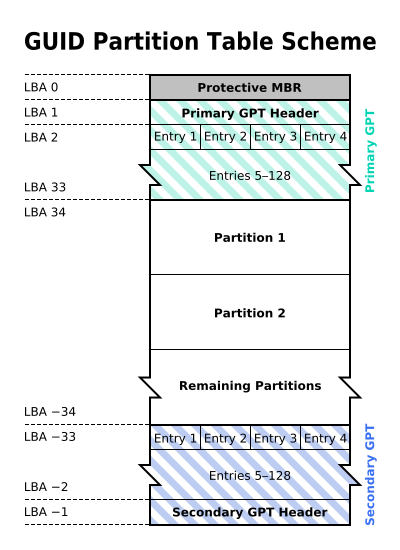
\includegraphics[width=40mm]{./src/img/gpt1.png}
        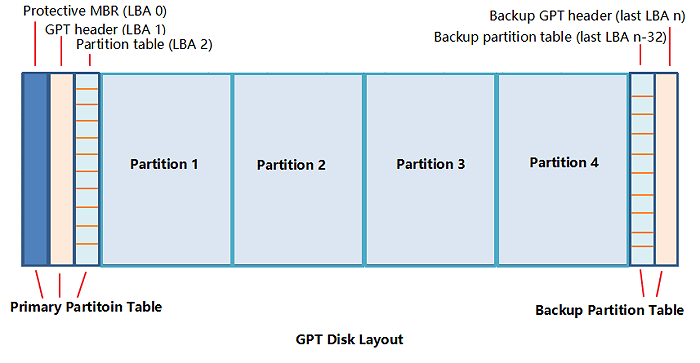
\includegraphics[width=75mm]{./src/img/gpt2.png}
        \caption{GPT Partition Table.}
        \label{fig:1}
    \end{center}
\end{figure}
\subsection{Partition Table}
\begin{enumerate}
    \item \textbf{Unmount FS!}
    \item \textbf{Create GPT partition table:}
\begin{Verbatim}[commandchars=\\\{\}]
\textcolor{root}{root#} \textcolor{command}{parted} -s <\textcolor{block}{/dev/sdX}> mktable gpt
\end{Verbatim}
\end{enumerate}
\subsection{Basic Partitions}
\begin{enumerate}
    \item \textbf{Enter cfdisk:}
\begin{Verbatim}[commandchars=\\\{\}]
\textcolor{root}{root#} \textcolor{command}{cfdisk} <\textcolor{block}{/dev/sdX}>
\end{Verbatim}
    \item \textbf{Create EFI partition (recommended 550 MiB):}
\begin{Verbatim}[commandchars=\\\{\}]
\textcolor{root}{cfdisk>} \textcolor{command}{n}
\textcolor{root}{cfdisk>} \textcolor{command}{550MiB}
\textcolor{root}{cfdisk>} \textcolor{command}{t}
\textcolor{root}{cfdisk>} \textcolor{command}{EFI System}
\end{Verbatim}
    \item \textbf{Create encrypted partition:}
\begin{Verbatim}[commandchars=\\\{\}]
\textcolor{root}{cfdisk>} \textcolor{command}{n}
\textcolor{root}{cfdisk>} \textcolor{command}{} (Enter)
\end{Verbatim}
    \item \textbf{Write changes:}
\begin{Verbatim}[commandchars=\\\{\}]
\textcolor{root}{cfdisk>} \textcolor{command}{W}
\textcolor{root}{cfdisk>} \textcolor{command}{yes}
\end{Verbatim}
    \item \textbf{Quit cfdisk:}
\begin{Verbatim}[commandchars=\\\{\}]
\textcolor{root}{cfdisk>} \textcolor{command}{Q}
\end{Verbatim}
    \item \textbf{Name partitions:}
\begin{Verbatim}[commandchars=\\\{\}]
\textcolor{root}{root#} \textcolor{command}{parted} -s <\textcolor{block}{/dev/sdX}> name 1 ESP
\textcolor{root}{root#} \textcolor{command}{parted} -s <\textcolor{block}{/dev/sdX}> name 2 LUKS
\end{Verbatim}
    \item \textbf{Format partitions:}
    \begin{enumerate}
        \item \textbf{ESP:}
\begin{Verbatim}[commandchars=\\\{\}]
\textcolor{root}{root#} \textcolor{command}{mkfs.fat} -F 32 <\textcolor{block}{/dev/sdX1}>
\textcolor{root}{root#} \textcolor{command}{fatlabel} <\textcolor{block}{/dev/sdX1}> <ESP>
\end{Verbatim}
        \item \textbf{LUKS:}
\begin{Verbatim}[commandchars=\\\{\}]
\textcolor{root}{root#} \textcolor{command}{cryptsetup} luksFormat --label <LUKS> <\textcolor{block}{/dev/sdX2}>
> YES
> <PASSWORD>
> <PASSWORD (VERIFY)>
\end{Verbatim}
    \end{enumerate}
\end{enumerate}
    \subsection{Advanced LUKS stuff}
\begin{itemize}
    \item \textbf{Open LUKS:}
\begin{Verbatim}[commandchars=\\\{\}]
\textcolor{root}{root#} \textcolor{command}{cryptsetup} open --type luks <\textcolor{block}{/dev/sdX2}> <luks>
> <PASSWORD>
\end{Verbatim}
    \item \textbf{Close LUKS:}
\begin{Verbatim}[commandchars=\\\{\}]
\textcolor{root}{root#} \textcolor{command}{cryptsetup} close <luks>
\end{Verbatim}
    \item \textbf{LUKS header:}
    \begin{enumerate}
        \item \textbf{See LUKS header:}
\begin{Verbatim}[commandchars=\\\{\}]
\textcolor{root}{root#} \textcolor{command}{cryptsetup} luksDump <\textcolor{block}{/dev/sdX2}>
\end{Verbatim}
        \item \textbf{Make LUKS header backup:}
\begin{Verbatim}[commandchars=\\\{\}]
\textcolor{root}{root#} \textcolor{command}{cryptsetup} luksHeaderBackup <\textcolor{block}{/dev/sdX2}>
--header-backup-file <\textcolor{file}{FILE}>
\end{Verbatim}
        \item \textbf{Destroy LUKS header:}
\begin{Verbatim}[commandchars=\\\{\}]
\textcolor{root}{root#} \textcolor{command}{cryptsetup} luksErase <\textcolor{block}{/dev/sdX2}>
> YES
\end{Verbatim}
        \item \textbf{Restore LUKS header:}
\begin{Verbatim}[commandchars=\\\{\}]
\textcolor{root}{root#} \textcolor{command}{cryptsetup} luksHeaderRestore <\textcolor{block}{/dev/sdX2}>
--header-backup-file <\textcolor{file}{FILE}>
> YES
\end{Verbatim}
    \end{enumerate}
    \item \textbf{Passwords}
    \begin{itemize}
        \item \textbf{Change password:}
\begin{Verbatim}[commandchars=\\\{\}]
\textcolor{root}{root#} \textcolor{command}{cryptsetup} luksChangeKey <\textcolor{block}{/dev/sdX2}>
> <OLD_PASSWORD>
> <NEW_PASSWORD>
> <NEW_PASSWORD (VERIFY)>
\end{Verbatim}
    \end{itemize}
\end{itemize}
\subsection{Encrypted Partition}
\begin{figure}[ht]
    \begin{center}
        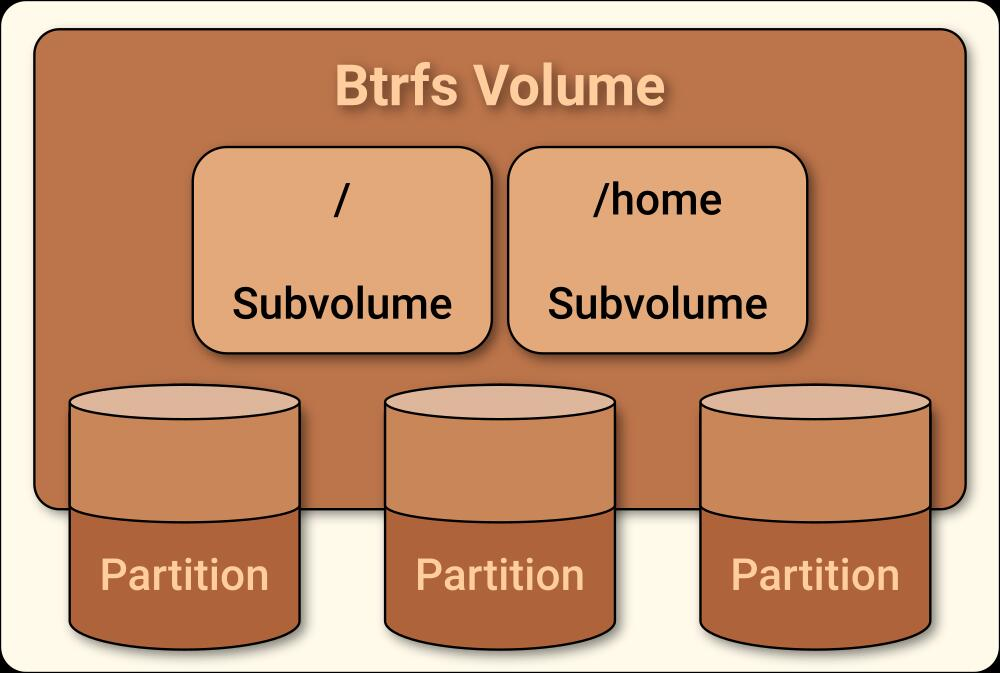
\includegraphics[width=75mm]{./src/img/btrfs.png}
        \caption{Btrfs structure.}
        \label{fig:1}
    \end{center}
\end{figure}
\begin{enumerate}
    \item \textbf{Open encrypted partition:}
\begin{Verbatim}[commandchars=\\\{\}]
\textcolor{root}{root#} \textcolor{command}{cryptsetup} open --type luks <\textcolor{block}{/dev/sdX2}> <luks>
> <PASSWORD>
\end{Verbatim}
    \item \textbf{Format root partition:}
\begin{Verbatim}[commandchars=\\\{\}]
\textcolor{root}{root#} \textcolor{command}{mkfs.btrfs} <\textcolor{block}{/dev/mapper/luks}>
\textcolor{root}{root#} \textcolor{command}{btrfs} filesystem label <\textcolor{block}{/dev/mapper/luks}> <GENTOO>
\end{Verbatim}
\end{enumerate}

\section{Stage3}
\begin{enumerate}
    \item \textbf{Mount Gentoo:}
\begin{Verbatim}[commandchars=\\\{\}]
\textcolor{root}{root#} \textcolor{command}{mount} <\textcolor{block}{/dev/mapper/luks}> <\textcolor{dir}{/mnt/gentoo/}>
\end{Verbatim}
    \item \textbf{Navigate to Gentoo install directory:}
\begin{Verbatim}[commandchars=\\\{\}]
\textcolor{root}{root#} \textcolor{command}{cd} <\textcolor{dir}{/mnt/gentoo/}>
\end{Verbatim}
    \item \textbf{Download Stage3 (from DK mirror):}
\begin{Verbatim}[commandchars=\\\{\}]
\textcolor{root}{root#} \textcolor{command}{links} https://www.gentoo.org/downloads/mirrors/
\end{Verbatim}
\menu[,]{DK, https://mirrors.dotsrc.org/gentoo/, releases/, amd64/, autobuilds/, current-stage3-amd64-openrc/, stage3-amd64-openrc-<release>.tar.xz}
    \item \textbf{Verify download: @todo}
    \item \textbf{Extract Stage3 tarball:}
\begin{Verbatim}[commandchars=\\\{\}]
\textcolor{root}{root#} \textcolor{command}{tar} xvJpf <\textcolor{file}{./stage3-amd64-openrc-<release>.tar.xz}>
--xattrs-include='*.*' --numeric-owner
\end{Verbatim}
    \item \textbf{Remove tar:}
\begin{Verbatim}[commandchars=\\\{\}]
\textcolor{root}{root#} \textcolor{command}{rm} -f <\textcolor{file}{./stage3-amd64-openrc-<release>.tar.xz}>
\end{Verbatim}
    \item \textbf{Copy Gentoo ebuild repository:}
\begin{Verbatim}[commandchars=\\\{\}]
\textcolor{root}{root#} \textcolor{command}{mkdir} -p \textcolor{dir}{/mnt/gentoo/etc/portage/repos.conf/}
\textcolor{root}{root#} \textcolor{command}{cp} \textcolor{file}{/mnt/gentoo/usr/share/portage/config/repos.conf}
\textcolor{file}{/mnt/gentoo/etc/portage/repos.conf/gentoo.conf}
\end{Verbatim}
\end{enumerate}

\section{Chroot}
\begin{enumerate}
    \item \textbf{Mount all filesystems:}
\begin{Verbatim}[commandchars=\\\{\}]
\textcolor{root}{root#} \textcolor{command}{mount} -t proc \textcolor{dir}{/proc/} <\textcolor{dir}{/mnt/gentoo/proc/}>
\textcolor{root}{root#} \textcolor{command}{mount} --rbind \textcolor{dir}{/sys/} <\textcolor{dir}{/mnt/gentoo/sys/}>
\textcolor{root}{root#} \textcolor{command}{mount} --make-rslave <\textcolor{dir}{/mnt/gentoo/sys/}>
\textcolor{root}{root#} \textcolor{command}{mount} --rbind \textcolor{dir}{/dev/} <\textcolor{dir}{/mnt/gentoo/dev/}>
\textcolor{root}{root#} \textcolor{command}{mount} --make-rslave <\textcolor{dir}{/mnt/gentoo/dev/}>
\textcolor{root}{root#} \textcolor{command}{mount} --bind \textcolor{dir}{/run/} <\textcolor{dir}{/mnt/gentoo/run/}>
\textcolor{root}{root#} \textcolor{command}{mount} --make-slave <\textcolor{dir}{/mnt/gentoo/run/}>
\end{Verbatim}
    \item \textbf{Chroot:}
\begin{Verbatim}[commandchars=\\\{\}]
\textcolor{root}{root#} \textcolor{command}{chroot} <\textcolor{dir}{/mnt/gentoo/}> \textcolor{file}{/bin/bash}
\textcolor{root}{root#} \textcolor{command}{source} \textcolor{file}{/etc/profile}
\textcolor{root}{root#} \textcolor{command}{export} PS1="(chroot) \$\{PS1\}"
\end{Verbatim}
    \item \textbf{Mount boot partition:}
\begin{Verbatim}[commandchars=\\\{\}]
\textcolor{root}{(chroot) root#} \textcolor{command}{mount} <\textcolor{block}{/dev/sdX1}> \textcolor{dir}{/boot/}
\end{Verbatim}
    \item \textbf{Add DNS:}
\begin{Verbatim}[commandchars=\\\{\}]
\textcolor{root}{(chroot) root#} \textcolor{command}{echo} "nameserver 1.1.1.1" > \textcolor{file}{/etc/resolv.conf}
\end{Verbatim}
\end{enumerate}

\section{Portage}
\begin{enumerate}
    \item \textbf{Find amount of available processing units:}
\begin{Verbatim}[commandchars=\\\{\}]
\textcolor{user}{(chroot) user\$} \textcolor{command}{nproc}
\end{Verbatim}
    \item \textbf{Configure compile options:}
\newline File (\textbf{\textcolor{file}{/etc/portage/make.conf}}):
\newline \url{https://github.com/AISK11/Gentoo/blob/main/configs/make.conf}
    \item \textbf{Create per-package license exceptions file:}
\begin{Verbatim}[commandchars=\\\{\}]
\textcolor{root}{(chroot) root#} \textcolor{command}{touch} \textcolor{file}{/etc/portage/package.license}
\end{Verbatim}
\end{enumerate}

\section{System Recompilation}
\begin{enumerate}
    \item \textbf{Synchronize repository:}
\begin{Verbatim}[commandchars=\\\{\}]
\textcolor{root}{(chroot) root#} \textcolor{command}{emerge} --sync
\end{Verbatim}
    \item \textbf{Read the news}
    \begin{itemize}
        \item \textbf{List all available news:}
\begin{Verbatim}[commandchars=\\\{\}]
\textcolor{root}{(chroot) root#} \textcolor{command}{eselect} news list
\end{Verbatim}
        \item \textbf{Read all/specific news:}
\begin{Verbatim}[commandchars=\\\{\}]
\textcolor{root}{(chroot) root#} \textcolor{command}{eselect} news read [N]
\end{Verbatim}
        \item \textbf{Purge all/specific news:}
\begin{Verbatim}[commandchars=\\\{\}]
\textcolor{root}{(chroot) root#} \textcolor{command}{eselect} news purge [N]
\end{Verbatim}
    \end{itemize}
    \item \textbf{Check selected profile:}
\newline Profile has to match downloaded Stage3 tarball!
    \begin{itemize}
        \item \textbf{See current profile:}
\begin{Verbatim}[commandchars=\\\{\}]
\textcolor{root}{(chroot) root#} \textcolor{command}{eselect} profile list
\end{Verbatim}
        \item \textbf{Change profile:}
\begin{Verbatim}[commandchars=\\\{\}]
\textcolor{root}{(chroot) root#} \textcolor{command}{eselect} profile set <N>
\end{Verbatim}
    \end{itemize}
    \item \textbf{Compile full system:}
\begin{Verbatim}[commandchars=\\\{\}]
\textcolor{root}{(chroot) root#} \textcolor{command}{emerge} -a --verbose --update --deep --newuse @world
\end{Verbatim}
\end{enumerate}

\section{System Packages}
\begin{enumerate}
    \item \textbf{Intel Microcode + Basic firmware (Intel microcode + iwlwifi):}
\newline File (\textbf{\textcolor{file}{/etc/portage/package.license}}):
\begin{Verbatim}[commandchars=\\\{\}]
sys-firmware/intel-microcode @BINARY-REDISTRIBUTABLE
sys-kernel/linux-firmware @BINARY-REDISTRIBUTABLE
\end{Verbatim}
\begin{Verbatim}[commandchars=\\\{\}]
\textcolor{root}{(chroot) root#} \textcolor{command}{emerge} -a sys-firmware/intel-microcode
sys-kernel/linux-firmware [app-admin/mcelog]
\end{Verbatim}
    \item \textbf{Filesystems (FAT32, LUKS, LVM2, BTRFS):}
\begin{Verbatim}[commandchars=\\\{\}]
\textcolor{root}{(chroot) root#} \textcolor{command}{emerge} -a sys-fs/dosfstools sys-fs/cryptsetup
sys-fs/btrfs-progs
\end{Verbatim}
    \item \textbf{UEFI:}
\begin{Verbatim}[commandchars=\\\{\}]
\textcolor{root}{(chroot) root#} \textcolor{command}{emerge} -a sys-boot/efibootmgr sys-boot/refind
\end{Verbatim}
    \item \textbf{Kernel + initramfs:}
\begin{Verbatim}[commandchars=\\\{\}]
\textcolor{root}{(chroot) root#} \textcolor{command}{emerge} -a sys-kernel/gentoo-sources sys-kernel/dracut
\end{Verbatim}
    \item \textbf{Network:}
\begin{Verbatim}[commandchars=\\\{\}]
\textcolor{root}{(chroot) root#} \textcolor{command}{emerge} -a net-misc/dhcpcd net-wireless/wpa_supplicant
\end{Verbatim}
\end{enumerate}

\section{Fstab}
\begin{enumerate}
    \item \textbf{Find UUIDs for block devices:}
\begin{Verbatim}[commandchars=\\\{\}]
\textcolor{root}{(chroot) root#} \textcolor{command}{blkid}
\end{Verbatim}
    \item \textbf{Configure fstab:}
\newline File (\textbf{\textcolor{file}{/etc/fstab}}):
\begin{Verbatim}[commandchars=\\\{\}]
\textcolor{comment}{## <disk UUID>                <mount>   <fs>  <options>     <dump> <pass>}
UUID=<UUID_/dev/sdX1>         /boot/    vfat  umask=0077              0 1
UUID=<UUID_/dev/mappper/luks> /         btrfs defaults,noatime,nofail 0 0
\end{Verbatim}
\end{enumerate}

\section{Kernel WIP}
\begin{enumerate}
    \item \textbf{Create linux kernel symlink:}
    \begin{enumerate}
        \item \textbf{List available kernels:}
\begin{Verbatim}[commandchars=\\\{\}]
\textcolor{root}{(chroot) root#} \textcolor{command}{eselect} kernel list
\end{Verbatim}
        \item \textbf{Create symlink}
\begin{Verbatim}[commandchars=\\\{\}]
\textcolor{root}{(chroot) root#} \textcolor{command}{eselect} kernel set <1>
\end{Verbatim}
    \end{enumerate}
    \item \textbf{Enter kernel configuration:}
\begin{Verbatim}[commandchars=\\\{\}]
\textcolor{root}{(chroot) root#} \textcolor{command}{cd} \textcolor{dir}{/usr/src/linux/} && \textcolor{command}{make} menuconfig
\end{Verbatim}
    \item \textbf{Configure kernel}
\newline \url{https://www.kernelconfig.io}
    \begin{enumerate}
\item \textbf{Gentoo:}
\begin{Verbatim}[commandchars=\\\{\}]
Gentoo Linux --->
   Generic Driver Options --->
      [*] Gentoo Linux support
      [*]   Linux dynamic and persistent device naming
          (userspace devfs) support
      [*]   Select options required by Portage features
        Support for init systems, system and service
        managers  --->
           [*] OpenRC, runit and other script based
              systems and managers
           [ ] systemd

Device Drivers --->
   Generic Driver Options --->
      -*- Maintain a devtmpfs filesystem to mount at /dev
      [*]   Automount devtmpfs at /dev, after the kernel
          mounted the rootfs
      SCSI device support  --->
         <*> SCSI disk support
\end{Verbatim}
        \item \textbf{CPU:}
\begin{Verbatim}[commandchars=\\\{\}]
Processor type and features  --->
   [*] Symmetric multi-processing support
   [*] Machine Check / overheating reporting
   [*]   Intel MCE features
   [ ]   AMD MCE features
   [*] CPU microcode loading support
   [*]   Intel microcode loading support
   [ ]   AMD microcode loading support

Binary Emulations --->
   [*] IA32 Emulation
\end{Verbatim}
        \item \textbf{Hard Drive:}
\begin{Verbatim}[commandchars=\\\{\}]
Device Drivers --->
   NVME Support --->
      <*> NVM Express block device
\end{Verbatim}
    \item \textbf{GPT:}
\begin{Verbatim}[commandchars=\\\{\}]
-*- Enable the block layer --->
   Partition Types --->
      [*] Advanced partition selection
      [ ] PC BIOS (MSDOS) partition tables) support
      [*] EFI GUID Partition support
\end{Verbatim}
        \item \textbf{Filesystems:}
\begin{Verbatim}[commandchars=\\\{\}]
File systems --->
   < > The Extended 4 (ext4) filesystem
   <*> Btrfs filesystem support
   DOS/FAT/EXFAT/NT Filesystems  --->
     <*> MSDOS fs support
     <*> VFAT (Windows-95) fs support
\end{Verbatim}
        \item \textbf{UEFI bootloader: WIP}
\begin{Verbatim}[commandchars=\\\{\}]
Processor type and features  --->
   [*] EFI runtime service support
   [*]   EFI stub support
   [*]     EFI mixed-mode support

Device Drivers --->
   Firmware Drivers  --->
      EFI (Extensible Firmware Interface) Support  --->
         <*> EFI Variable Support via sysfs

File systems  --->
   Pseudo filesystems  --->
      <*> EFI Variable filesystem

Device Drivers --->
   Graphics support --->
      Frame buffer Devices --->
         <*> Support for frame buffer devices --->
            [*] EFI-based Framebuffer Support
\end{Verbatim}
        \item \textbf{Initramfs:}
\begin{Verbatim}[commandchars=\\\{\}]
General setup  --->
   [*] Initial RAM filesystem and RAM disk (initramfs/initrd) support
Device Drivers --->
   Generic Driver Options --->
      [*] Maintain a devtmpfs filesystem to mount at /dev
\end{Verbatim}
        \item \textbf{LUKS: WIP}
\begin{Verbatim}[commandchars=\\\{\}]
[*] Enable loadable module support

Device Drivers --->
  [*] Multiple devices driver support (RAID and LVM) --->
    <*> Device mapper support
      <*> Crypt target support

[*] Cryptographic API --->
    <*> XTS support
    -*- SHA224 and SHA256 digest algorithm
    -*- AES cipher algorithms

General setup  --->
    [*] Initial RAM filesystem and RAM disk (initramfs/initrd) support
??
[*] Cryptographic API --->
    <*> User-space interface for hash algorithms
    <*> User-space interface for symmetric key cipher algorithms
\end{Verbatim}
        \item \textbf{RAID: WIP}
\begin{Verbatim}[commandchars=\\\{\}]
Device Drivers  --->
   Multiple devices driver support (RAID and LVM)  --->
       < > RAID support
\end{Verbatim}
        \item \textbf{LVM: WIP}
\begin{Verbatim}[commandchars=\\\{\}]
Device Drivers  --->
   Multiple devices driver support (RAID and LVM)  --->
       <*> Device mapper support
           <*> Crypt target support
           <*> Snapshot target
           <*> Mirror target
           <*> Multipath target
               <*> I/O Path Selector based on the number of in-flight I/Os
               <*> I/O Path Selector based on the service time
\end{Verbatim}
        \item \textbf{USB: TEST}
\begin{Verbatim}[commandchars=\\\{\}]
Device Drivers --->
  HID support  --->
    -*- HID bus support
    <*>   Generic HID driver
    [*]   Battery level reporting for HID devices
      USB HID support  --->
        <*> USB HID transport layer
  [*] USB support  --->
    <*>     xHCI HCD (USB 3.0) support
    <*>     EHCI HCD (USB 2.0) support
    <*>     OHCI HCD (USB 1.1) support
\end{Verbatim}
        \item \textbf{WiFi: TEST}
\begin{Verbatim}[commandchars=\\\{\}]
[*] Networking support  --->
    [*] Wireless  --->
        <M>   cfg80211 - wireless configuration API
        [*]     enable powersave by default
        <M>   Generic IEEE 802.11 Networking Stack (mac80211)
        -*-   Enable LED triggers

Device Drivers  --->
        [*] Network device support  --->
        --- Network device support
        [*]   Wireless LAN  --->
            --- Wireless LAN
            [*]   Intel devices
            <M>     Intel Wireless WiFi Next Gen AGN -
                    Wireless-N/Advanced-N/Ultimate-N (iwlwifi)
            <M>       Intel Wireless WiFi DVM Firmware support
            <M>       Intel Wireless WiFi MVM Firmware support
\end{Verbatim}
    \end{enumerate}
    \item \textbf{Compile kernel:}
\begin{Verbatim}[commandchars=\\\{\}]
\textcolor{root}{(chroot) root#} \textcolor{command}{cd} \textcolor{dir}{/usr/src/linux/} && \textcolor{command}{make} && \textcolor{command}{make} modules_install
\end{Verbatim}
    \item \textbf{Copy kernel to boot dir:}
\begin{Verbatim}[commandchars=\\\{\}]
\textcolor{root}{(chroot) root#} \textcolor{command}{cd} \textcolor{dir}{/usr/src/linux/} && \textcolor{command}{make} install
\end{Verbatim}
\end{enumerate}

\section{Initramfs WIP}
\begin{enumerate}
    \item \textbf{Find compiled kernels:}
\begin{Verbatim}[commandchars=\\\{\}]
\textcolor{root}{(chroot) root#} \textcolor{command}{ls} \textcolor{dir}{/boot/}
\end{Verbatim}
    \item \textbf{List all available modules:}
\begin{Verbatim}[commandchars=\\\{\}]
\textcolor{root}{(chroot) root#} \textcolor{command}{dracut} --kver <5.15.26-gentoo> --list-modules
\end{Verbatim}
    \item \textbf{Generate initramfs [and show included modules]:}
\begin{Verbatim}[commandchars=\\\{\}]
\textcolor{root}{(chroot) root#} \textcolor{command}{dracut} --kver <5.15.26-gentoo> --kernel-cmdline="root=/dev/sda2" -f
[-M 2> \textcolor{block}{/dev/null}]

--early-microcode ?

---- PARAMS -----
dracut
</boot/initramfs-5.15.26-gentoo.img>
--kver <5.15.26-gentoo>
-f
-m "
i18n
btrfs
crypt
dm
kernel-modules
kernel-modules-extra
resume
rootfs-block
terminfo
udev-rules
usermount
base
fs-lib
shutdown
"
--kernel-cmdline"
rd.shell
[rd.vconsole.keymap=de-latin1-nodeadkeys]
[rd.vconsole.font=eurlatgr]
[rd.locale.LANG=pl_PL.utf8]
[rd.locale.LC_ALL=]
rd.luks.uuid=<UUID_/dev/sda2>
root=UUID=<UUID_/dev/mapper/luks>
rootfstype=btrfs
rootflags=defaults,noatime,nofail
"
[--early-microcode]
-M 2> /dev/null




dracut </boot/initramfs-5.15.26-gentoo.img> --kver <5.15.26-gentoo> -H
--fstab /etc/fstab -f -M -L 3





rd.luks=1 rd.lvm=0 rd.md=0 rd.dm=0 (or omit modules)

rd.shell

dracut --print-cmdline

rd.luks.uuid=luks-c00...399 root=/dev/mapper/luks rootfstype=btrfs rootflags=rw,relatime,space_cache=v2,subvolid=5,subvol=/


\end{Verbatim}
    \item \textbf{Check initramfs content:}
\begin{Verbatim}[commandchars=\\\{\}]
\textcolor{root}{(chroot) root#} \textcolor{command}{lsinitrd} <\textcolor{file}{/boot/initramfs-<5.15.26-gentoo>.img}>
\end{Verbatim}
\end{enumerate}

\section{Bootloader WIP}
\begin{enumerate}
    \item \textbf{System must be booted fro UEFI:}
\begin{Verbatim}[commandchars=\\\{\}]
\textcolor{root}{(chroot) root#} \textcolor{command}{dmesg} | \textcolor{command}{grep} -i efi
\end{Verbatim}
    \item \textbf{Generate rEFInd entry:}
\begin{Verbatim}[commandchars=\\\{\}]
\textcolor{root}{(chroot) root#} \textcolor{command}{refind-install}

edit /boot/refi*
quiet root=/dev/mapper/luks-<UUID_/dev/mapper/luks>

\end{Verbatim}
\end{enumerate}

\section{Local System Settings}
See section \ref{section:local_settings}

\section{Finishing WIP}


\chapter{Local Settings WIP}
\label{section:local_settings}
\section{Hostname}
\begin{itemize}
    \item \textbf{Print [full] hostname:}
\begin{Verbatim}[commandchars=\\\{\}]
\textcolor{user}{user\$} \textcolor{command}{hostname} [-f]
\end{Verbatim}
    \item \textbf{Change hostname:}
    \begin{enumerate}
        \item \textbf{Change hostname permanently:}
\newline File (\textbf{\textcolor{file}{/etc/hostname}}):
\begin{verbatim}
<HOSTNAME>
\end{verbatim}
    \item \textbf{Reboot PC to take effect:}
\begin{Verbatim}[commandchars=\\\{\}]
\textcolor{root}{root#} \textcolor{command}{reboot}
\end{Verbatim}
    \end{enumerate}
\end{itemize}

\section{Date \& Time}
\subsection{Timezone}
\begin{itemize}
    \item \textbf{Show current timezone:}
\newline Has to be created during installation.
\begin{Verbatim}[commandchars=\\\{\}]
\textcolor{user}{user\$} \textcolor{command}{cat} \textcolor{file}{/etc/timezone}
\end{Verbatim}
    \item \textbf{Change timezone:}
    \begin{enumerate}
        \item \textbf{See available timezones:}
\newline Directory (\textbf{\textcolor{dir}{/usr/share/zoneinfo/}}).
        \item \textbf{Set timezone:}
\begin{Verbatim}[commandchars=\\\{\}]
\textcolor{root}{root#} \textcolor{command}{echo} "<Europe/Copenhagen>" > \textcolor{file}{/etc/timezone}
\textcolor{root}{root#} \textcolor{command}{emerge} --config sys-libs/timezone-data
\end{Verbatim}
    \end{enumerate}
\end{itemize}
\subsection{System Clock}
\label{section:date}
\begin{itemize}
    \item \textbf{Show system time:}
    \begin{itemize}
        \item \textbf{Default:}
\begin{Verbatim}[commandchars=\\\{\}]
\textcolor{user}{user\$} \textcolor{command}{date}
\end{Verbatim}
        \item \textbf{ISO 8601 (YYYY-MM-DDThh:mm:ss(+|-)xx:xx):}
\begin{Verbatim}[commandchars=\\\{\}]
\textcolor{user}{user\$} \textcolor{command}{date} +'\%Y-\%m-\%dT\%H:\%M:\%S\%:z'
\end{Verbatim}
    \end{itemize}
    \item \textbf{Set system time:}
    \begin{itemize}
        \item \textbf{Manually:}
\begin{Verbatim}[commandchars=\\\{\}]
\textcolor{root}{root#} \textcolor{command}{date} <MMDDhhmmYYYY>
\end{Verbatim}
        \item \textbf{With NTP/PTP @todo}
    \end{itemize}
\end{itemize}
\subsection{Hardware Clock (RTC)}
\begin{itemize}
    \item \textbf{Display RTC:}
\begin{Verbatim}[commandchars=\\\{\}]
\textcolor{root}{root#} \textcolor{command}{hwclock}
\end{Verbatim}
    \item \textbf{Update RTC with system clock:}
\begin{Verbatim}[commandchars=\\\{\}]
\textcolor{root}{root#} \textcolor{command}{hwclock} --systohc
\end{Verbatim}
\end{itemize}

\section{Locales}
\begin{itemize}
    \item \textbf{See locales:}
\begin{Verbatim}[commandchars=\\\{\}]
\textcolor{user}{user\$} \textcolor{command}{locale}
\end{Verbatim}
    \item \textbf{Set locales:}
    \begin{enumerate}
        \item \textbf{List available locales:}
\begin{Verbatim}[commandchars=\\\{\}]
\textcolor{user}{user\$} \textcolor{command}{cat} \textcolor{file}{/usr/share/i18n/SUPPORTED}
\end{Verbatim}
        \item \textbf{Generate locales:}
\newline File (\textbf{\textcolor{file}{/etc/locale-gen}}):
\newline \url{https://github.com/AISK11/Gentoo/blob/main/configs/locale-gen}
\begin{Verbatim}[commandchars=\\\{\}]
\textcolor{root}{root#} \textcolor{command}{locale-gen}
\end{Verbatim}
    \item \textbf{List available generated locales:}
\begin{Verbatim}[commandchars=\\\{\}]
\textcolor{user}{user\$} \textcolor{command}{locale} -a
\end{Verbatim}
    \item \textbf{Set system locales:}
\newline File (\textbf{\textcolor{file}{/etc/env.d/02locale}}):
\newline \url{https://github.com/AISK11/Gentoo/blob/main/configs/02locale}
    \item \textbf{Use changed locales:}
\begin{Verbatim}[commandchars=\\\{\}]
\textcolor{root}{root#} \textcolor{command}{env-update} && \textcolor{command}{source} \textcolor{file}{/etc/profile}
\end{Verbatim}
    \end{enumerate}
\end{itemize}

\section{Console Keyboard}
\begin{enumerate}
    \item \textbf{See all available keyboards:}
\newline File (\textbf{\textcolor{file}{/etc/env.d/02locale}}):
\newline Directory (\textbf{\textcolor{dir}{/usr/share/keymaps/i386/}}).
    \item \textbf{Set keyboard:}
\newline File: (\textbf{\textcolor{file}{/etc/conf.d/keymaps}}):
\begin{verbatim}
keymap="us"
\end{verbatim}
\end{enumerate}

\chapter{Portage}
\begin{itemize}
    \item eselect [news]
    \item emerge
    \item layman?
\end{itemize}


% https://wiki.gentoo.org/wiki/Handbook:AMD64/Installation/Base
% https://wiki.gentoo.org/wiki/Localization/Guide#Environment_variables_for_locales
% https://wiki.archlinux.org/title/Locale
% https://www.gnu.org/software/libc/manual/html_node/Locale-Categories.html#index-LC_005fTIME





% ToDo:
% Locale + CLI keyboard, font, etc
% Kernel + initramfs
% efibootmgr + rEFInd
% runit
% ZSH
% xen
% SELINUX
% hardened kernel

% Networking
% Portage + Pentoo

% System hardening (nftables, usbguard, no motd, ulimits, ...)

\section{Help Me}
\url{https://forums.gentoo.org/viewtopic-t-1147683.html}
\url{https://wiki.gentoo.org/wiki/Full_Encrypted_Btrfs/Native_System_Root_Guide}

\section{Future Reads}
\url{https://wiki.gentoo.org/wiki/SELinux/Tutorials/The_security_context_of_a_process}
\url{https://wiki.gentoo.org/wiki/Hardened/Introduction_to_Hardened_Gentoo}
\url{https://wiki.gentoo.org/wiki/Xen}

\chapter{ToDo}
\begin{itemize}
    \item \textbf{perfect kernel, dracut and rEFInd}
    \item \textbf{Finish installation (root password, locales)}
    \item \textbf{Select and configure init process}
    \item \textbf{zsh + vim}
    \item \textbf{Portage + Pentoo}
    \item \textbf{Networking}
    \item \textbf{System cleaning}
    \item \textbf{System hardening}
    \item \textbf{Xen}
    \item \textbf{look at hardened ans SELinux}
\end{itemize}

\end{document}
